\documentclass[journal,12pt,onecolumn]{IEEEtran}
\usepackage{cite}
 \usepackage{caption}
\usepackage{graphicx}
\usepackage{amsmath,amssymb,amsfonts,amsthm}
\usepackage{algorithmic}
\usepackage{graphicx}
\usepackage{textcomp}
\usepackage{xcolor}
\usepackage{txfonts}
\usepackage{listings}
\usepackage{enumitem}
\usepackage{mathtools}
\usepackage{gensymb}
\usepackage{comment}
\usepackage[breaklinks=true]{hyperref}
\usepackage{tkz-euclide} 
\usepackage{listings}
\usepackage{gvv}
%\def\inputGnumericTable{}                                 
\usepackage[latin1]{inputenc} 
\usetikzlibrary{arrows.meta, positioning}
\usepackage{xparse}
\usepackage{color}                                            
\usepackage{array}                                            
\usepackage{longtable}                                       
\usepackage{calc}                                             
\usepackage{multirow}
\usepackage{multicol}
\usepackage{hhline}                                           
\usepackage{ifthen}                                           
\usepackage{lscape}
\usepackage{tabularx}
\usepackage{array}
\usepackage{float}

\usepackage{float}
%\newcommand{\define}{\stackrel{\triangle}{=}}
\theoremstyle{remark}
\usepackage{circuitikz}
\captionsetup{justification=centering}
\usepackage{tikz}

\title{Matrices in Geometry 10.5.3}
\author{EE25BTECH11035 - Kushal B N}
\begin{document}
\vspace{3cm}
\maketitle
{\let\newpage\relax\maketitle}
\textbf{Question: }
Draw a pair of tangents to a circle of radius $5cm$ which are inclined to each other at an angle of $60\degree$.

\textbf{Solution: }\\
Let the center be the origin. Then the circle with radius $5cm$ is
\begin{equation}
    \vec{C} : \vec{x}^{\top}\vec{V}\vec{x} + 2\vec{u}^{\top}\vec{x} + f = 0
\end{equation}
where,
\begin{equation}
    \vec{V} = \myvec{1&0\\0&1} \text{ , } \vec{u} = \myvec{0\\0} \text{ , } f = -25
\end{equation}

Let the tangents be drawn from an external point $\vec{h}$.
Line segment from $O$ to $h$ bisects the angle between the tangents and it forms two right angled triangles.
So that, we have
\begin{equation}
    \sin{\frac{60\degree}{2}} = \frac{r}{\norm{\vec{h}}} = \frac{5}{\norm{\vec{h}}}
\end{equation}

\begin{equation}
    \implies \norm{\vec{h}} = \frac{5}{\sin{30\degree}} = 10
\end{equation}

So the point $h$ should be at a distance of $10cm$ from the origin(centre).
Let the point be
\begin{equation}
    \vec{h} = \myvec{10\\0}
\end{equation}

Calculating the matrix $\Sigma$
\begin{equation}
    \Sigma = (\vec{V}\vec{h} + \vec{u})(\vec{V}\vec{h} + \vec{u})^{\top} - g(\vec{h})\vec{V}
\end{equation}

\begin{equation}
    g(\vec{h}) = \vec{h}^{\top}\vec{V}\vec{h} + 2\vec{u}^{\top}\vec{h} + f = \norm{\vec{h}}^2 + f = 100 - 25 = 75
\end{equation}

\begin{equation}
    \Sigma = \vec{h}\vec{h}^{\top} - g(\vec{h})\vec{V} = \myvec{10\\0}\myvec{10&0} - 75\myvec{1&0\\0&1}
\end{equation}

\begin{equation}
    \implies \Sigma = \myvec{25&0\\0&-75}
\end{equation}
The eigen values of the matrix $\Sigma$ are 
\begin{equation}
    \lambda_1 = 25
\end{equation}

\begin{equation}
    \lambda_2 = -75
\end{equation}
The direction vectors for the tangents
\begin{equation}
    \myvec{\sqrt{\abs{\lambda_2}}\\ \pm \sqrt{\abs{\lambda_1}}} = \myvec{5\sqrt{3}\\ \pm 5}
\end{equation}

\begin{equation}
    \implies \vec{m}_1 = \myvec{\sqrt{3}\\1} \text{ , } \vec{m}_2 = \myvec{\sqrt{3}\\-1}
\end{equation}
As the tangents pass through $\vec{h}$ with direction vectors $\vec{m}_1$ and $\vec{m}_2$, using the normal form of the line $\vec{n}^{\top}(\vec{x}-\vec{h}) = 0$.
Their equations are
\begin{equation}
    \myvec{1&-\sqrt{3}}\brak{\vec{x} - \myvec{10\\0}} = 0
\end{equation}

\begin{equation}
    \myvec{1&\sqrt{3}}\brak{\vec{x} - \myvec{10\\0}} = 0
\end{equation}

\textbf{Plot: }\\

\begin{figure}[H]
    \centering
    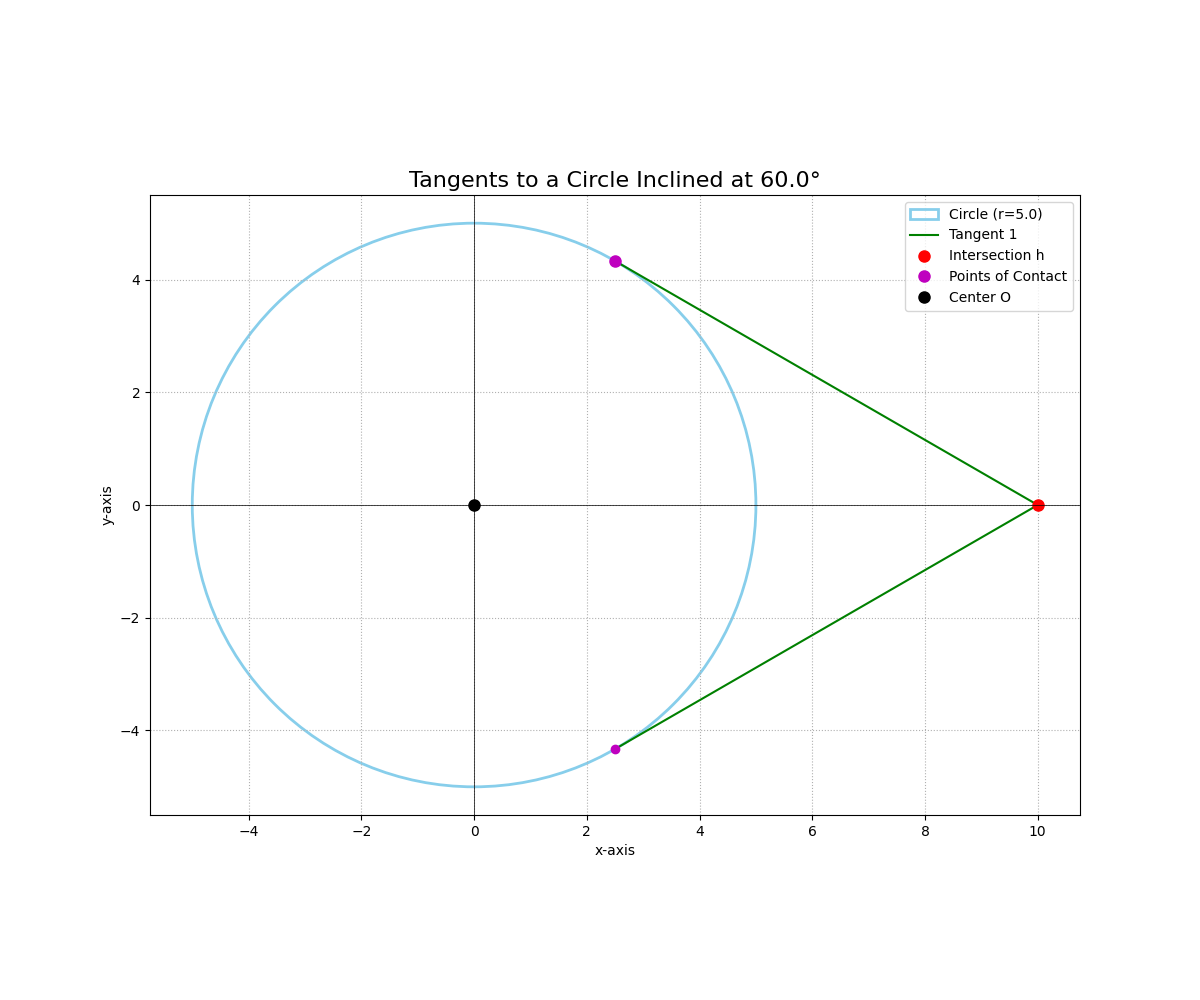
\includegraphics[width=0.80\columnwidth]{figs/1.png}
    \caption{Plot for 10.5.3}
\end{figure}
\end{document}
